\begin{frame}[fragile]
  \frametitle{课程主旨}
  \begin{center}
  {\Huge 为“疯狂”点赞\\
    \vspace{0.5cm}
    为科学“正名”}\\
  \vspace{1cm}
  {\Large 正史书王迹,稗官言秘闻。\\
    \vspace{0.2cm}
    % 万般皆杳杳,唯有醉中真。}
    万般皆杳杳,莫辨假与真。}
\end{center}
\end{frame}

\begin{frame}
  \frametitle{科学}
  \begin{block}{科学(science)}
科学(science)的基本特征是其方法论:对世界的认识源于观测或实验的信息(或者数据),总结信息时会形成模型(亦称假说或理论),模型会指导进一步的探索,直到遇到这些模型无法解释的现象,这就导致对这些模型的更新和替代。这就是科学的方法。只有用科学的方法进行的探索才能称为科学。
  \end{block}
\end{frame}

\begin{frame}
  \frametitle{四大}
  \vspace{-0.5em}
  \begin{figure}
    \centering
    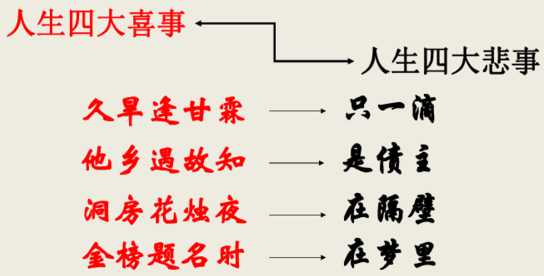
\includegraphics[width=0.5\textwidth]{c0_four.jpg}
  \end{figure}
  \vspace{-0.5em}
  \begin{block}{人生四大喜事}
    久旱逢甘雨,他乡遇故知。洞房花烛夜,金榜题名时。
  \end{block}
  \pause
  \begin{block}{世界四大不可抗力}
    猫咪总能四脚着地,面包涂着果酱的那面总是先落地,旁边的队伍总是比你的快,蚊子不会被洗澡水砸死。
  \end{block}
\end{frame}

\begin{frame}
  \frametitle{研究实例}
  \begin{block}{胡立德研究成果}
    \begin{itemize}
      \item 【2003年8月Nature封面】很多昆虫在水面行走主要是依靠在水表面产生波纹的表面张力
      \item 【2005年9月Nature封面】昆虫“坐电梯”爬上岸
      \item 【PNAS(美国国家科学院院刊),2015年菠萝科学奖】蚊子因体重较轻而在雨滴的碰撞中得以生存
      \item 【PNAS(美国国家科学院院刊),2015年搞笑诺贝尔奖】排尿定律:所有哺乳动物排空膀胱所用的时间是一致的,大约是21秒
      \item 无论什么哺乳动物,平均的睫毛长度都恰是眼长的1/3,这恰好是保持角膜滋润并避开灰尘的最理想的长度
      \item 火蚁在水中会形成筏子,相当于是一种能自修复材料的材料
      \item 火蚁可以像液体一样流动
    \end{itemize}
  \end{block}
\end{frame}

\begin{frame}
  \frametitle{科研立项}
    \begin{table}
    \centering
    \rowcolors[]{1}{blue!20}{blue!10}
    \begin{tabular}{cl}
      \hline
      \rowcolor{blue!50}资助金额/万 & 研究名称\\
      \hline
      1300 & 猴子和黑猩猩喜欢什么类型的音乐?\\
      500 & 喝醉的鸟唱歌的时候是不是也会大舌头?\\
      390 & 什么会让金鱼觉得很有X吸引力?\\
      350 & 为什么耶稣的脸会出现在烤面包上?\\
      290 & 谁会是美国下一任超模?\\
      260 & 政治上的自由主义是后天选择还是基因决定的?\\
      190 & 你能跑得过恐龙吗?\\
      110 & {\footnotesize 拉拉队员组成拉拉队之后,会不会比她们一个人时看起来更漂亮?}\\
      100 & 被被蜜蜂叮了以后,哪儿最疼?\\
      100 & 为什么打哈欠会传染?\\
      \hline
    \end{tabular}
  \end{table}
\end{frame}

\begin{frame}
  \frametitle{科研立项(续)}
    \begin{table}
    \centering
    \rowcolors[]{1}{blue!20}{blue!10}
    \begin{tabular}{cl}
      \hline
      \rowcolor{blue!50}资助金额/万 & 研究名称\\
      \hline
      85.5 & 吃虫子的时候,民主党人会感到更恶心,还是共和党人?\\
      75.3 & 松鼠的毛比较多,还是雄蜂的毛比较多?\\
      17.2 & 为什么端着咖啡走路会让咖啡洒出来?\\
      56 & 大学生最喜欢在短信里用什么表情?\\
      51.1 & 脸书是不是令人成瘾?\\
      39 & 湿漉漉的狗要甩多少次才能把自己甩干?\\
      34 & 黑猩猩游戏是不是打得比人好?\\
      33.1 & 像赛马那样尿尿,需要多长时间?\\
      24.3 & 可卡因是否能让蜜蜂跳舞?\\
      5 & 民主党人和共和党人相貌是否不同?\\
      \hline
    \end{tabular}
  \end{table}
\end{frame}

\begin{frame}
  \frametitle{参考教材}
  \begin{figure}
    \centering
    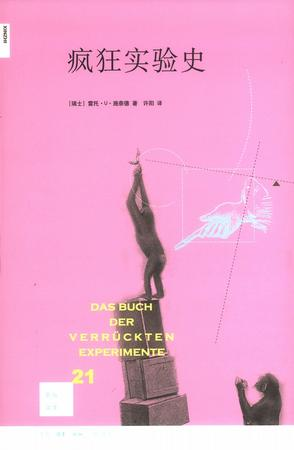
\includegraphics[width=5cm]{c0_book_01.jpg}
    \qquad
    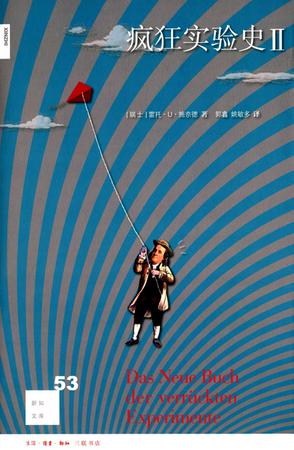
\includegraphics[width=5cm]{c0_book_02.jpg}
  \end{figure}
\end{frame}

\begin{frame}
  \frametitle{课外读物}
  \begin{figure}
    \centering
    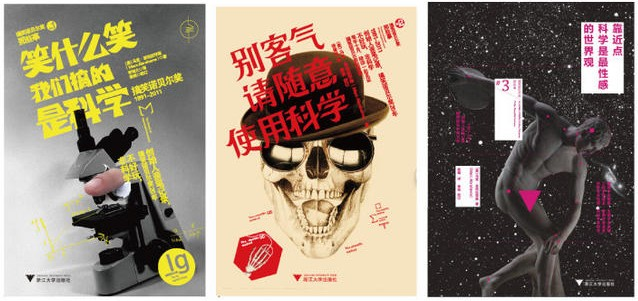
\includegraphics[width=11cm]{c0_book_03.jpg}
  \end{figure}
\end{frame}

\begin{frame}
  \frametitle{课外读物}
  \begin{figure}
    \centering
    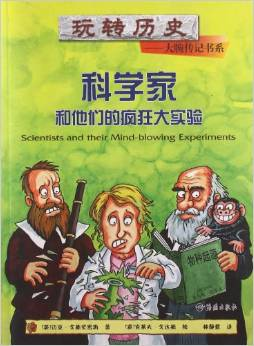
\includegraphics[width=2.7cm]{c0_book_04.jpg}\quad
    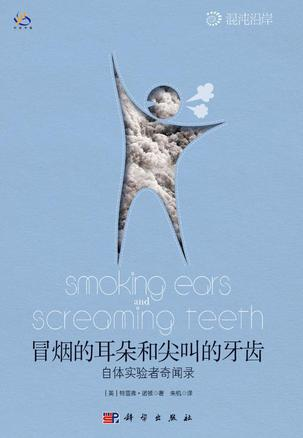
\includegraphics[width=2.55cm]{c0_book_05.jpg}\quad
    
\includegraphics[width=2.8cm]{c0_book_06.jpg}\\
    
\includegraphics[width=2.8cm]{c0_book_07.jpg}\hspace{1cm}
    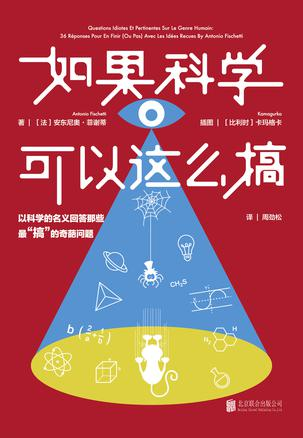
\includegraphics[width=2.8cm]{c0_book_08.jpg}
  \end{figure}
\end{frame}

\begin{frame}
  \frametitle{授课资料}
  \begin{figure}
    \centering
    
\includegraphics[width=0.55\textwidth]{qr.png}
  \end{figure}
  \begin{center}
  \href{https://github.com/Yixf-Education/course_Crazy_Experiment}{https://github.com/Yixf-Education/course\_Crazy\_Experiment}
  \end{center}
\end{frame}

% \begin{frame}
%   \frametitle{短片视频}
%   \begin{figure}
%     \centering
%     
\includegraphics[width=0.55\textwidth]{c0_short_movie.png}
%   \end{figure}
%   \begin{center}
%     \href{http://www.tudou.com/listplay/YUwEELLXLoI.html}{http://www.tudou.com/listplay/YUwEELLXLoI.html}
%   \end{center}
% \end{frame}

% \begin{frame}
%   \frametitle{实验视频}
%   \begin{figure}
%     \centering
%     
\includegraphics[width=0.55\textwidth]{c0_experiment.png}
%   \end{figure}
%   \begin{center}
%     \href{http://www.tudou.com/listplay/eGZ9cyk2Ejs.html}{http://www.tudou.com/listplay/eGZ9cyk2Ejs.html}
%   \end{center}
% \end{frame}

\begin{frame}
  \frametitle{课程安排}
  \begin{center}
  \alert{前8周,每周四,晚上两节(18:00-19:40),西楼603}\\
  \vspace{0.2cm}
  \end{center}
  \begin{block}{授课内容}
    \begin{itemize}
      \item 物理学、化学、心理学、生物学、医学、……
      \item 谈天说地,评古论今
    \end{itemize}
  \end{block}
\end{frame}

\begin{frame}
  \frametitle{\alert{考核方式}}
  \begin{block}{考勤}
    \begin{itemize}
      \item 不点名,但随机提问
      \item 缺勤0次——优秀(及以下)
      \item 缺勤1次——良好(及以下)
      \item 缺勤2次——及格(及以下)
      \item \alert{缺勤3次——不及格}
    \end{itemize}
  \end{block}
  \pause
  \begin{block}{报告}
    \begin{itemize}
      \item 内容:自己关于某个(疯狂)实验的简单设想
      \item 要求:电子版,~500字(一页纸),含灵感来源、实验目的、基本方案等;\alert{抄袭——不及格}
      \item 提交:\alert{yixfbio@gmail.com},\alert{课程名-学号-姓名-共享/保密.doc}
      \item 示例:在Word里面撰写 $\rightarrow$ 重命名为“疯狂的实验-201600-张三-共享.doc” $\rightarrow$ 发送邮件 $\rightarrow$ 等待回复
    \end{itemize}
  \end{block}
\end{frame}

